\section{Test Program}
We were supplied with the following test program:
\begin{verbatim}
00: lw r1, 1(r0) -- Data: 2
01: lw r1, 2(r0) -- Data: 10
02: lw r1, 2(r0) -- Data: 10
03: add r3, r1, r2
04: sw r3, 5(r0)
05: beq r0, r0, 2
06: sw r3, 3(r0)
07: sw r3, 4(r0)
08: sw r3, 6(r0)
09: sw r3, 7(r0)
10: lui r3, 6
11: sw r3, 8(r0)
12: add r3, r1, r3
13: sw r3, 9(r0)
14: beq r0, r0, -3
15: sw r3, 10(r0)
\end{verbatim}



\section{Simulation}

\begin{figure}[ht]
    \centering
    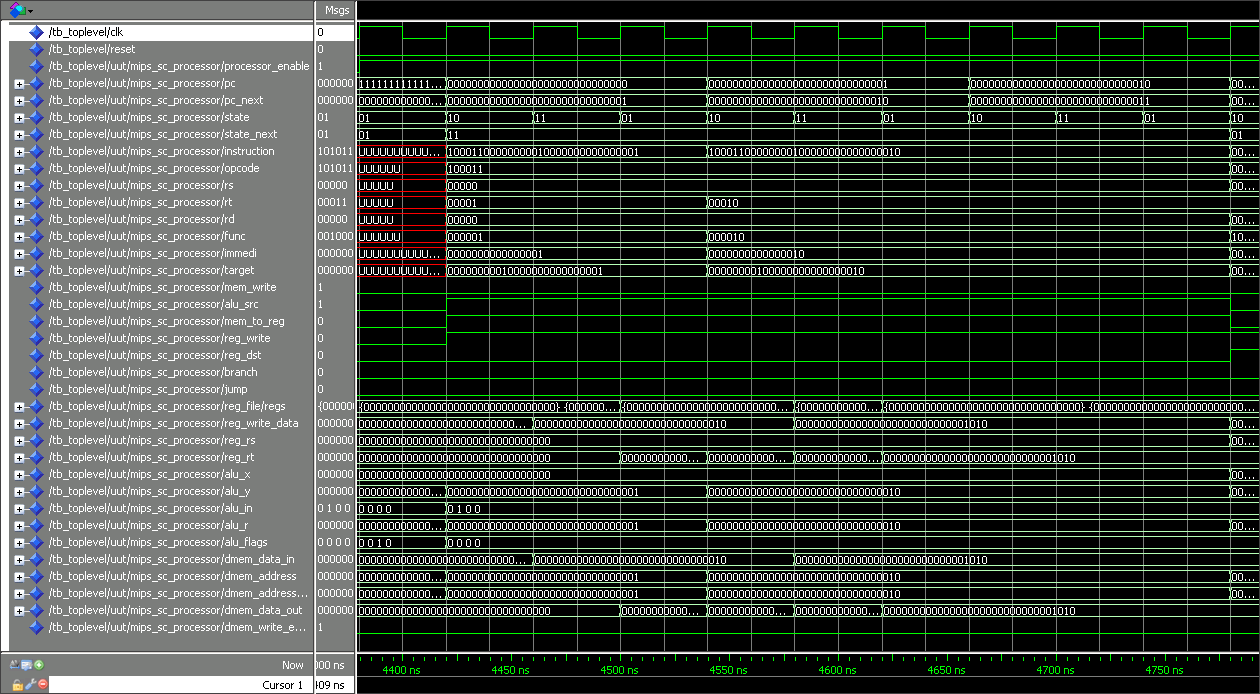
\includegraphics[scale=0.3]{figures/sim1.png}
    \caption{\label{fig:sim1}Simulation Part 1 - Instruction 0,1,2}
\end{figure}

\begin{figure}[ht]
    \centering
    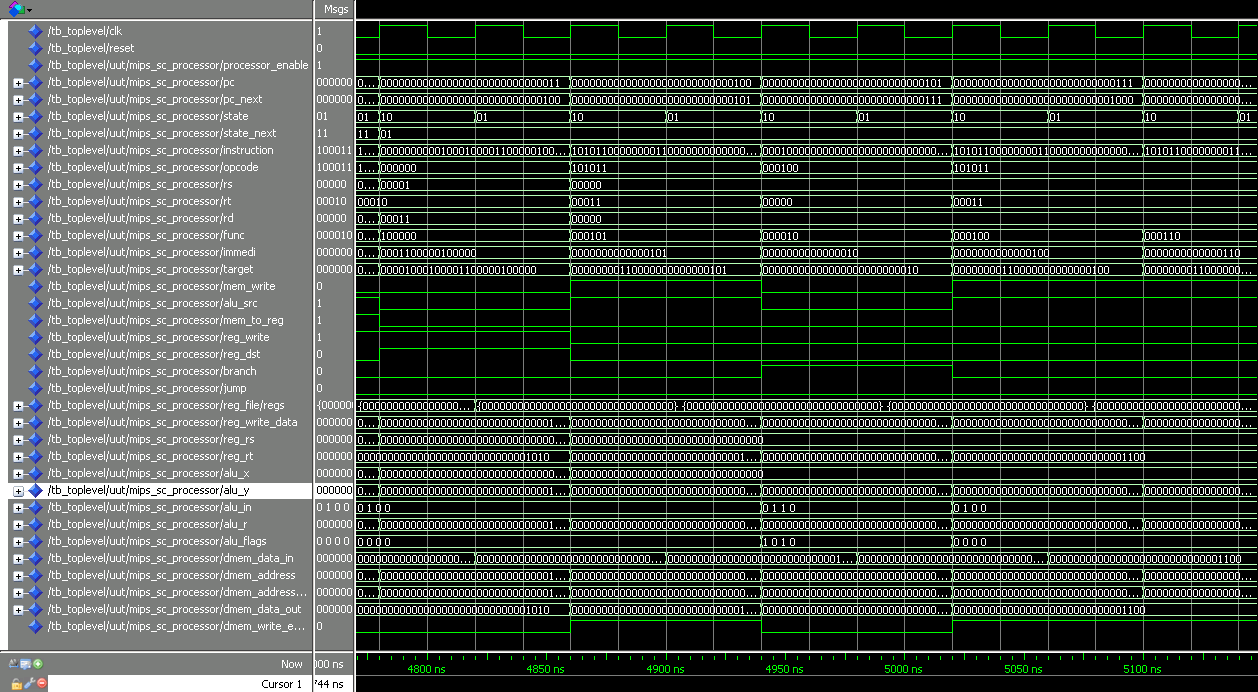
\includegraphics[scale=0.3]{figures/sim2.png}
    \caption{\label{fig:sim2}Simulation Part 2 - Instuction 3,4,5,7}
\end{figure}

\begin{figure}[ht]
    \centering
    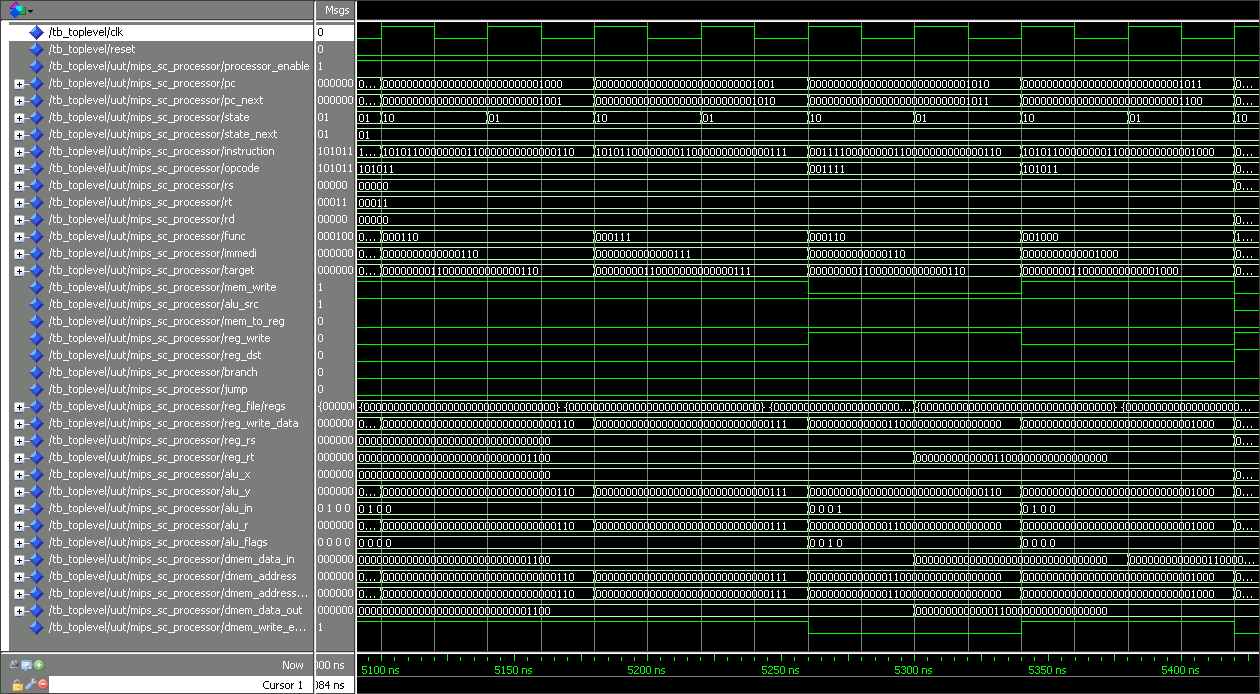
\includegraphics[scale=0.3]{figures/sim3.png}
    \caption{\label{fig:sim3}Simulation Part 3 - Instruction 8,9,10,11}
\end{figure}

\begin{figure}[ht]
    \centering
    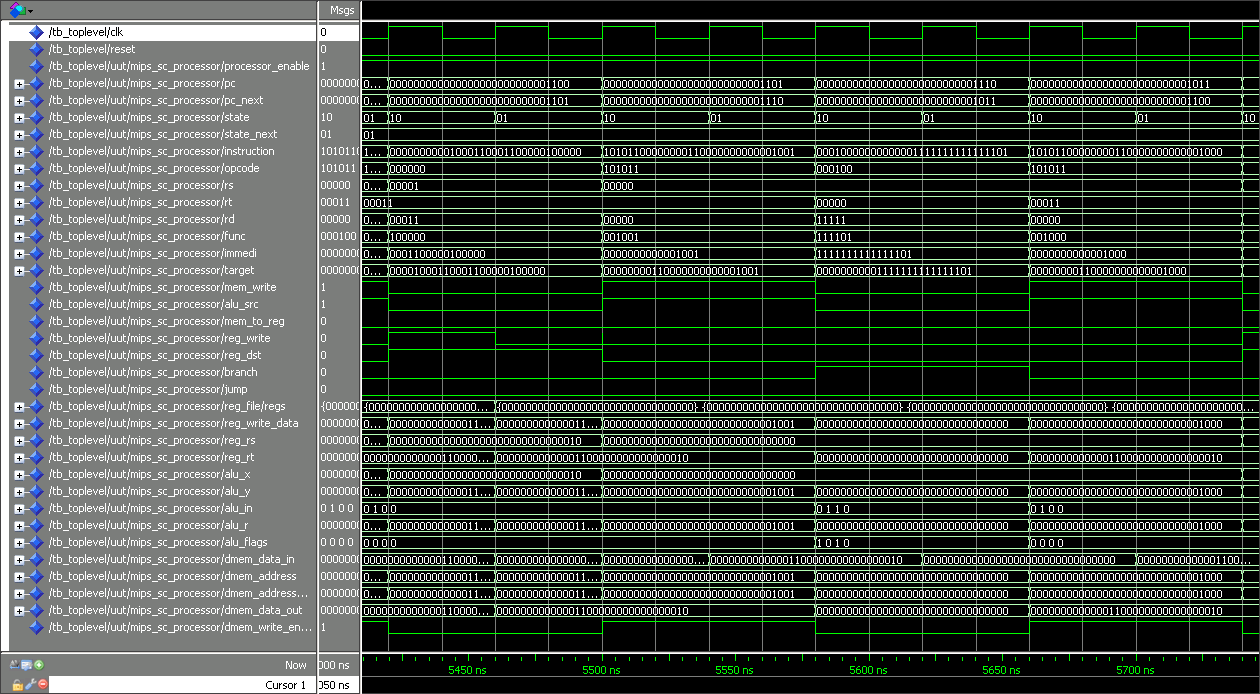
\includegraphics[scale=0.3]{figures/sim4.png}
    \caption{\label{fig:sim4}Simulation Part 4 - Instruction 12,13,14,11}
\end{figure}

